\section{模型评价}
\subsection{模型的主要优势}
本文从物理约束的一致性、所得方案的可验证性、最优性结论的适用范围和对输入误差的承受能力四个方面评价模型。四问的目标和约束逐步增加：问题一不考虑实体设备竞争，问题二加入运输机与电池周转，问题三再加入连续通信，问题四固定第三问任务后考察独立分组。因此，不宜仅凭架次数或总能耗的增减判断后一个模型是否优于前一个模型；应首先确认每问所对应的可行域和评价口径。

模型的首要优点是将地形、载荷、能源和时间约束贯通到四问，而不是分别构造互不兼容的计算口径。问题一利用DEM确定航段爬升高度，按载荷递减计算往返能耗和安全载荷；问题二沿用同一航段物理量形成多点候选路线，并把运输机返航与电池充满视为不同的资源释放事件；问题三在既定运输轨迹上引入中继机的飞行、建链、悬停和周转；问题四读取已经验证的任务区间和通信保障关系进行分组。这样，后一问增加约束时可以回溯到前一问的航段、架次或资源区间，结果变化具有明确的来源。

分层求解使不同规模的子问题采用与其结构相符的方法。问题一的单区组批用状态压缩动态规划求解，最优性仅对应单点往返及其字典序目标。问题二先筛除不满足质量、体积、返航电量或即时硬时限的路线，再对有限候选池进行货箱覆盖和共享资源排程；固定已选24条路线后的整数秒时序目标值与求解下界同为4281382。问题三用有限宽度搜索形成候选，随后对正式方案作物理回代和连续通信证明。问题四的依赖图只产生三个不可拆单元，因而可穷尽两组的三种划分和三组的一种划分。表~\ref{tab:model-eval-scope}把这些不同强度的结论并列，避免把局部最优性或可行性验证误写成四问联合全局最优。

\begin{table}[htbp]
\centering\small
\caption{四问结果的主要验证依据及其结论范围}
\label{tab:model-eval-scope}
\begin{tabular}{@{}p{0.10\textwidth}p{0.43\textwidth}p{0.39\textwidth}@{}}
\toprule
问题 & 可核查依据 & 可支持的结论\\
\midrule
一 & 安全载荷求根、可行组批枚举与动态规划回溯 & 单点往返模型下的组批最优\\
二 & 80箱逐箱回代、双资源区间核查；固定路线整数模型目标值等于下界 & 正式排程可行；已选路线的整数时序最优\\
三 & 80箱交付与四类资源回代；1317个区间覆盖全部36198.242\,s通信需求 & 给定DEM、轨迹及链路预算下全时段通信可行\\
四 & 连续证书提取任务依赖；全部四种无标号分区逐一计算 & 固定第三问任务下的分区比较穷尽\\
\bottomrule
\end{tabular}
\end{table}

可行性检验也比单一目标值更完整。第二问逐箱核对唯一交付和硬时限，并分别检查运输机、电池占用；第三问除了最大间隔1\,s的事件采样，还对分段仿射轨迹和题给DEM建立连续时间区间证书。证书中未决区间为零，因此结论不依赖于“采样点之间大概不会掉线”的假设。第四问使用证书中实际选用的中继保障边，而不是把候选中继点可能覆盖的所有服务区都强行并组，减少了对分区可行域的过度限制。这些回代与证书使模型输出能够从货箱、架次、通信区间逐级检查。

模型还能把资源瓶颈转化为可执行的配置判断。问题二中A、B、C型运输机和电池的并发峰值均达到库存，说明只按架次数配置而忽略充电周转会低估资源需求。问题四进一步指出：保持第三问时刻表和保障关系时，两组独立执行至少缺1架C型机和1块C型电池，三组则各缺2件；缺口来自跨组不能继续共享C型资源，而非中继能源组件数量不足。该结论直接回答了现有设备能否支撑独立救援组，以及需要补充何种设备。

\subsection{结果验证与安全裕量}
模型的另一优势是把“求得方案”与“验证方案”分开。第二问对80箱逐一复算交付时刻，并检查运输机和电池的具体占用区间；第三问以连续时间区间证书覆盖全部36198.242\,s通信需求，而不是只在有限采样点检验链路；第四问再从该证书提取实际使用的中继关系，验证分组后的任务归属和设备峰值。表~\ref{tab:model-eval-scope}中的证书与回代记录使每一步都可追溯，也明确了各问结论的强度。

在可行性之外，时间和通信裕量用于判断方案接近哪些边界。问题三的\texttt{S002}医疗和饮用水箱恰在3600\,s硬截止时刻交接；连续通信证书的最小保守链路裕量下界为0.008976\,dB。这两个指标并不否定已完成的时限与通信验证，而是帮助识别后续需要优先保留缓冲的任务和链路区间。以下图表直接取自逐箱结果和连续证书，分别展示紧约束的位置及其分布。

为避免只用极小值概括全体结果，图~\ref{fig:model-eval-hard-slack}从具有硬截止时刻的31箱中，选出问题三余量最小的8箱，并与同箱在问题二的余量对照。\texttt{S002}两箱由问题二的550.684\,s余量降至零，直接展示了联合通信调度之后的时间紧张点；其余箱仍有正余量。这是两份\emph{已求得方案}的逐箱比较，不是对延误扰动的重新求解实验。
\begin{figure}[htbp]
\centering
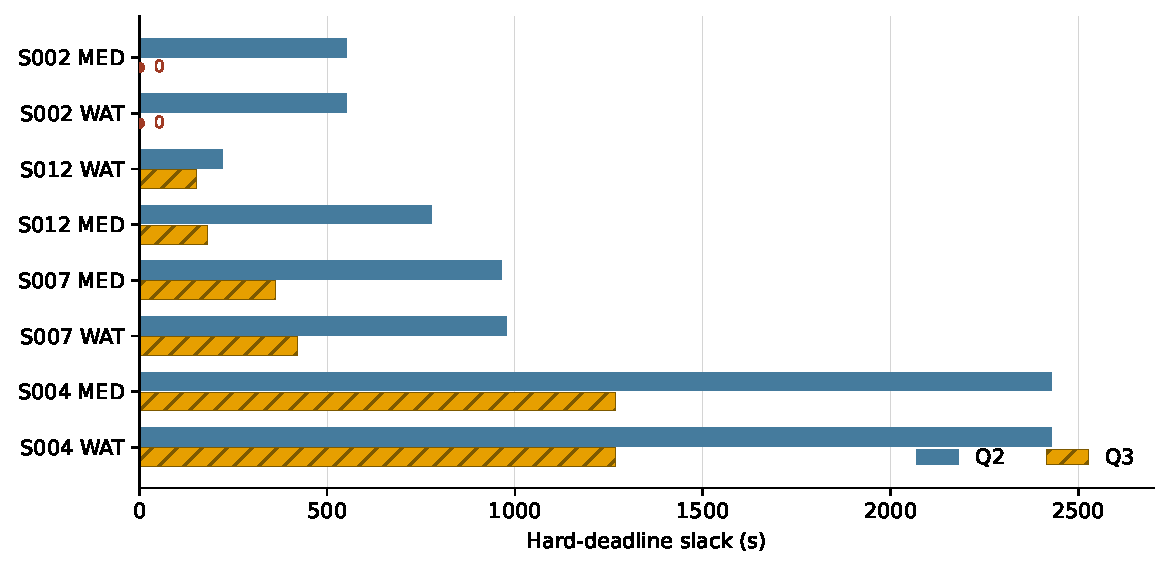
\includegraphics[width=0.90\textwidth]{figures/model_eval_hard_slack.pdf}
\caption{问题三余量最小的8个硬时限箱在问题二、三中的交付余量；数据取自两问逐箱结果，零余量仍满足硬约束}
\label{fig:model-eval-hard-slack}
\end{figure}

图~\ref{fig:model-eval-link-margin}则按证明区间统计1317个保守链路裕量下界：其中127个区间低于1\,dB，最小为0.008976\,dB。图中的频数以\emph{区间个数}为单位，不以服务时长加权；它说明边界裕量不只由一个孤立采样点产生，但不能据此推断现场掉线概率或具体可容忍的定位误差。
\begin{figure}[htbp]
\centering
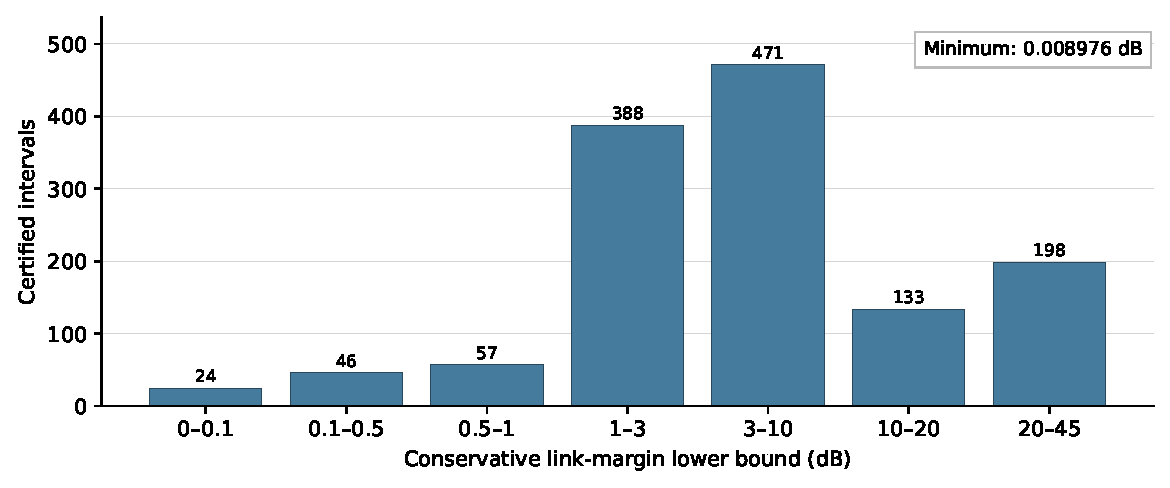
\includegraphics[width=0.90\textwidth]{figures/model_eval_link_margin.pdf}
\caption{问题三连续通信证书的保守链路裕量下界分布；各柱为已证区间数量，非独立实验重复次数}
\label{fig:model-eval-link-margin}
\end{figure}

进一步对同一正式方案作单因素保守敏感性检查：保持运输时刻、中继任务和证书选定的通信提供者不变，假设每条已用链路的路径损耗均额外增加$\Delta L$。若区间$I$原有的保守裕量下界满足$m_I-\Delta L\geq\varepsilon_L$，原区间证明仍成立；$\varepsilon_L$沿用连续证书的数值保护量。按区间时长加权，原证书可直接保留的需求时间比例为
\[
R(\Delta L)=\frac{\sum_{I:m_I-\Delta L\geq\varepsilon_L}|I|}{\sum_I|I|}.
\]
图~\ref{fig:model-eval-loss-stress}给出$0$--$5$\,dB附加损耗下的计算结果：增加1\,dB时，原证书仍覆盖90.4\%的需求时间；增加3\,dB时为61.3\%。由于最小裕量不足0.01\,dB，任何超过该值的统一附加损耗都使\emph{原证书}无法再覆盖全部时段。未保留证明的区间可能改由其他提供者保障，因此曲线既不是实际在线率，也不是重排任务后的最优覆盖率。
\begin{figure}[htbp]
\centering
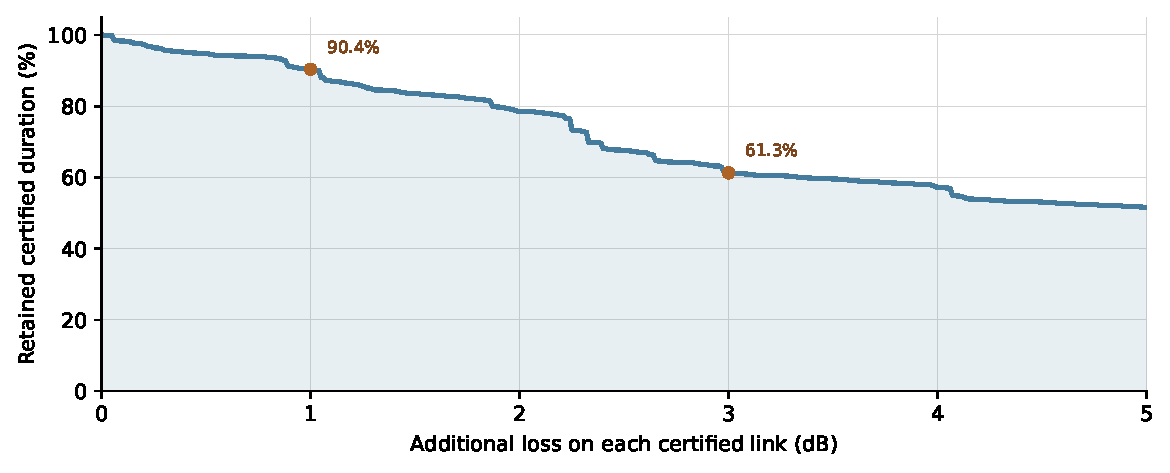
\includegraphics[width=0.90\textwidth]{figures/model_eval_loss_stress.pdf}
\caption{固定问题三时刻和已选通信提供者时，附加统一路径损耗后的原证书保留时长比例；未保留区间仅表示需要重新证明}
\label{fig:model-eval-loss-stress}
\end{figure}

\subsection{适用范围与结果复核}
本文的数值结论针对题给15个服务区、80个不可拆货箱、现有运输与中继设备、固定网关及所给DEM。运输路线、交付时刻和通信证书使用同一套地形与设备参数，但四问的输入依赖并不相同：问题一的安全载荷提供单架次物理边界，问题二选出的运输排程是问题三的起点，问题四又以问题三的正式任务和已选保障关系为固定基线。若服务区位置、设备性能、地形或通信参数发生变化，应从受影响的上游环节重新计算，不能直接沿用本题的24条运输路线、5条中继任务或三个不可拆分组。

结果复核也应遵循这一依赖次序。先用航段数据重算路线的载荷、飞行时间、能耗与返航电量，再核对逐箱交付和运输机、电池的占用区间；对第三问，还需检查中继机与组件占用、回传链路及连续证书是否覆盖全部运输通信需求，不能用离散采样记录替代区间证明；最后才根据证书中实际使用的中继关系重建第四问依赖图，并重新计算各组设备峰值。项目结果目录分别保存第二问的逐箱记录、第三问的正式解与连续证书、第四问的分区枚举结果，使每一级结论都能对应到原始计算记录。此复核链条检验的是模型内一致性，不等同于现场试飞或无线传播实测。

\subsection{局限与改进方向}
现有方案的边界主要有两点：问题二的候选路线与问题三的中继点、束搜索状态未穷尽全部可能，因此相应正式方案是经验证的可行解，不宣称全局最优；航时、能耗、充电和链路参数按题给值确定，图~\ref{fig:model-eval-hard-slack}和图~\ref{fig:model-eval-link-margin}所示的紧约束需要在实际部署前留出更充分的余量。这些边界不影响前述模型内可行性与第四问固定任务分区的穷尽性。

后续可先以最小硬时限余量和最小链路裕量为次级指标，联动细化运输时刻、中继服务窗及悬停位置，再用现有的逐箱、资源与连续通信证书重新验收。若需要更强的最优性结论，可按排程瓶颈扩充候选路线与中继点，并为路线选择及资源调度构造有效下界。若独立救援组优先于沿用问题三任务表，则可把组间隔离要求提前纳入联合调度。各项改进都能沿用本文的物理计算和分层验证框架，但新增性能应以重新求解后的结果报告。
